\documentclass[varwidth]{standalone}
\usepackage{tikz}
\usetikzlibrary{external}
\usetikzlibrary{arrows}
\usepackage{pgfplots}
\pgfplotsset{compat=1.16}
\usepgfplotslibrary{smithchart}

\definecolor{HB9UFblue}{RGB}{0,61,165}
\definecolor{HB9UFred}{HTML}{ED135A}

\begin{document}
\begin{tikzpicture}
    \begin{smithchart}[clip=false]
      \pgfplotsset{yticklabel in circle}
      \pgfplotsset{ticks=none}
% \addplot[thick,smooth,color=HB9UFblue] table[x index = {3}, y index = {4}] {schwingkreis.dat};
%     \fill [fill=black] (axis cs:1,0) circle [radius=2pt];
%     \node [below left]  at  (axis cs:1,0) {$f_r$};
      \addplot[thick,smooth,color=HB9UFblue,->] table[x index = {0}, y index = {1}] {Rseriell.dat};
      \addplot[thick,smooth,color=HB9UFblue,->] table[x index = {2}, y index = {3}] {Rseriell.dat};
      \addplot[thick,smooth,color=HB9UFblue,->] table[x index = {4}, y index = {5}] {Rseriell.dat};
      \addplot[thick,smooth,color=HB9UFblue,->] table[x index = {6}, y index = {7}] {Rseriell.dat};
      \addplot[thick,smooth,color=HB9UFblue,->] table[x index = {8}, y index = {9}] {Rseriell.dat};
      \node[fill=white,anchor=north west] at (current bounding box.north west) {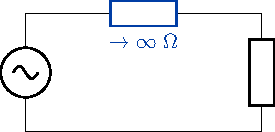
\includegraphics[width=2cm]{Rseriell.pdf}};
      \node[fill=white,anchor=south west] at (current bounding box.south west) {(a)};
  \end{smithchart}
\end{tikzpicture}
\begin{tikzpicture}
    \begin{smithchart}[smithchart mirrored,ticks=none]
    \end{smithchart}
    \begin{smithchart}[ticks=none,grid style={transparent},clip=false]
      \pgfplotsset{ticks=none}
      \addplot[thick,smooth,color=HB9UFblue,->] table[x index = {0}, y index = {1}] {Rparallel.dat};
      \addplot[thick,smooth,color=HB9UFblue,->] table[x index = {2}, y index = {3}] {Rparallel.dat};
      \addplot[thick,smooth,color=HB9UFblue,->] table[x index = {4}, y index = {5}] {Rparallel.dat};
      \addplot[thick,smooth,color=HB9UFblue,->] table[x index = {6}, y index = {7}] {Rparallel.dat};
      \addplot[thick,smooth,color=HB9UFblue,->] table[x index = {8}, y index = {9}] {Rparallel.dat};
      \node[fill=white,anchor=north west] at (current bounding box.north west) {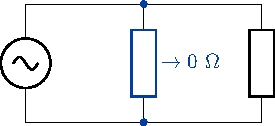
\includegraphics[width=2cm]{Rparallel.pdf}};
      \node[fill=white,anchor=south west] at (current bounding box.south west) {(b)};
  \end{smithchart}
\end{tikzpicture}

\begin{tikzpicture}
    \begin{smithchart}[clip=false]
      \pgfplotsset{yticklabel in circle}
      \pgfplotsset{ticks=none}
      \addplot[thick,smooth,color=HB9UFblue,->] table[x index = {0}, y index = {1}] {Lseriell.dat};
      \addplot[thick,smooth,color=HB9UFblue,->] table[x index = {2}, y index = {3}] {Lseriell.dat};
      \addplot[thick,smooth,color=HB9UFblue,->] table[x index = {4}, y index = {5}] {Lseriell.dat};
      \addplot[thick,smooth,color=HB9UFblue,->] table[x index = {6}, y index = {7}] {Lseriell.dat};
      \addplot[thick,smooth,color=HB9UFblue,->] table[x index = {8}, y index = {9}] {Lseriell.dat};
      \addplot[thick,smooth,color=HB9UFblue,->] table[x index = {10}, y index = {11}] {Lseriell.dat};
      \addplot[thick,smooth,color=HB9UFblue,->] table[x index = {12}, y index = {13}] {Lseriell.dat};

      \addplot[thick,smooth,color=HB9UFred,dashed,->] table[x index = {0}, y index = {1}] {Cseriell.dat};
      \addplot[thick,smooth,color=HB9UFred,dashed,->] table[x index = {2}, y index = {3}] {Cseriell.dat};
      \addplot[thick,smooth,color=HB9UFred,dashed,->] table[x index = {4}, y index = {5}] {Cseriell.dat};
      \addplot[thick,smooth,color=HB9UFred,dashed,->] table[x index = {6}, y index = {7}] {Cseriell.dat};
      \addplot[thick,smooth,color=HB9UFred,dashed,->] table[x index = {8}, y index = {9}] {Cseriell.dat};
      \addplot[thick,smooth,color=HB9UFred,dashed,->] table[x index = {10}, y index = {11}] {Cseriell.dat};
      \addplot[thick,smooth,color=HB9UFred,dashed,->] table[x index = {12}, y index = {13}] {Cseriell.dat};
      \node[fill=white,anchor=north west] at (current bounding box.north west) {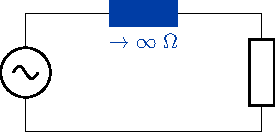
\includegraphics[width=2cm]{Lseriell.pdf}\hspace{5mm}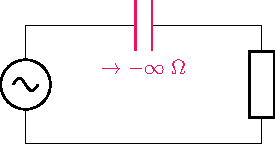
\includegraphics[width=2cm]{Cseriell.pdf}};
      \node[fill=white,anchor=south west] at (current bounding box.south west) {(c)};
  \end{smithchart}
\end{tikzpicture}
\begin{tikzpicture}
    \begin{smithchart}[smithchart mirrored,ticks=none]
    \end{smithchart}
    \begin{smithchart}[ticks=none,grid style={transparent},clip=false]
      \pgfplotsset{ticks=none}
      \addplot[thick,smooth,color=HB9UFblue,->] table[x index = {0}, y index = {1}] {Lparallel.dat};
      \addplot[thick,smooth,color=HB9UFblue,->] table[x index = {2}, y index = {3}] {Lparallel.dat};
%     \addplot[thick,smooth,color=HB9UFblue,->] table[x index = {4}, y index = {5}] {Lparallel.dat};
      \addplot[thick,smooth,color=HB9UFblue,->] table[x index = {6}, y index = {7}] {Lparallel.dat};
      \addplot[thick,smooth,color=HB9UFblue,->] table[x index = {8}, y index = {9}] {Lparallel.dat};
      \addplot[thick,smooth,color=HB9UFblue,->] table[x index = {10}, y index = {11}] {Lparallel.dat};
      \addplot[thick,smooth,color=HB9UFblue,->] table[x index = {12}, y index = {13}] {Lparallel.dat};

      \addplot[thick,smooth,color=HB9UFred,dashed,->] table[x index = {0}, y index = {1}] {Cparallel.dat};
      \addplot[thick,smooth,color=HB9UFred,dashed,->] table[x index = {2}, y index = {3}] {Cparallel.dat};
%     \addplot[thick,smooth,color=HB9UFred,dashed,->] table[x index = {4}, y index = {5}] {Cparallel.dat};
      \addplot[thick,smooth,color=HB9UFred,dashed,->] table[x index = {6}, y index = {7}] {Cparallel.dat};
      \addplot[thick,smooth,color=HB9UFred,dashed,->] table[x index = {8}, y index = {9}] {Cparallel.dat};
      \addplot[thick,smooth,color=HB9UFred,dashed,->] table[x index = {10}, y index = {11}] {Cparallel.dat};
      \addplot[thick,smooth,color=HB9UFred,dashed,->] table[x index = {12}, y index = {13}] {Cparallel.dat};
      \node[fill=white,anchor=north west] at (current bounding box.north west) {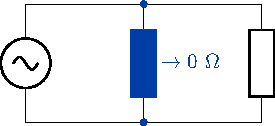
\includegraphics[width=2cm]{Lparallel.pdf}\hspace{5mm}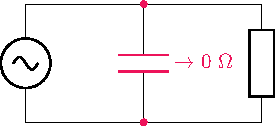
\includegraphics[width=2cm]{Cparallel.pdf}};
      \node[fill=white,anchor=south west] at (current bounding box.south west) {(d)};
  \end{smithchart}
\end{tikzpicture}

\begin{tikzpicture}
    \begin{smithchart}[clip=false]
      \pgfplotsset{yticklabel in circle}
      \pgfplotsset{ticks=none}
      \addplot[thick,smooth,color=HB9UFblue,->] table[x index = {0}, y index = {1}] {TL50.dat};
      \addplot[thick,smooth,color=HB9UFblue,->] table[x index = {2}, y index = {3}] {TL50.dat};
      \addplot[thick,smooth,color=HB9UFblue,->] table[x index = {4}, y index = {5}] {TL50.dat};
      \addplot[thick,smooth,color=HB9UFblue,->] table[x index = {6}, y index = {7}] {TL50.dat};
      \addplot[thick,smooth,color=HB9UFblue,->] table[x index = {8}, y index = {9}] {TL50.dat};

      \addplot[thick,smooth,color=HB9UFred,dashed,->] table[x index = {0}, y index = {1}] {TL100.dat};
      \node[fill=white,anchor=north west] at (current bounding box.north west) {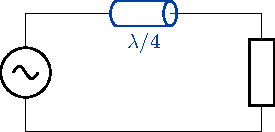
\includegraphics[width=2cm]{TL.pdf}};
      \node[fill=white,anchor=south west] at (current bounding box.south west) {(e)};
  \end{smithchart}
\end{tikzpicture}
\begin{tikzpicture}
    \begin{smithchart}[clip=false]
      \pgfplotsset{yticklabel in circle}
      \pgfplotsset{ticks=none}
      \addplot[thick,smooth,color=HB9UFblue,->] table[x index = {0}, y index = {1}] {LTL.dat};
      \node[fill=white,anchor=north west] at (current bounding box.north west) {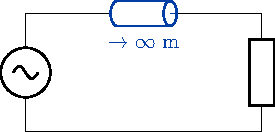
\includegraphics[width=2cm]{LTL.pdf}};
      \node[fill=white,anchor=south west] at (current bounding box.south west) {(f)};
  \end{smithchart}
\end{tikzpicture}
\end{document}
